\chapter{IoT Gateway}\label{chap:iotgateway}

Unser Internet of Things Gateway besteht wiederum aus mehreren Teilen. Die einzelnen Sensoren werden entweder über den CAN-Bus oder an ein Sming angeschlossen. Der CAN-Bus wird von uns über ein BeagleBone Cape mitgelesen. Die Daten des Smings können wir ebenfalls auf dem BeagleBone empfangen. Dies erreichen wir mit Hilfe des Bluetooth Smart USB Dongle BLED112 von Bluegiga, welcher am BeagleBone angeschlossen wird.

\begin{figure}[hbtp]
    \center
    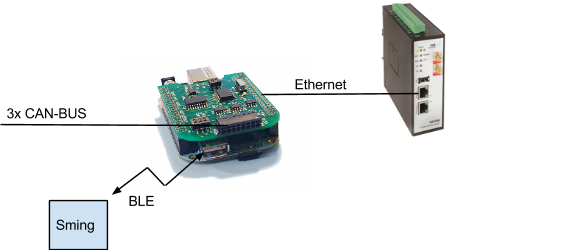
\includegraphics[width=\textwidth]{bilder/aufbau_in_auto.png}
    \caption{Aufbau des IoT Gateways}
    \label{fig:aufbau_iot_gateway}
\end{figure}

\section{Netmodule NetBox NB1600}\label{sec:netbox}
Um die Verbindung zur Cloud zu ermöglichen, setzen wir die bereits vom Sming Projekte bekannte NetBox NB1600 ein. Für uns kommt sie als mobiler 3G/4G Router zum Einsatz.

\begin{figure}[hbtp]
	\center
	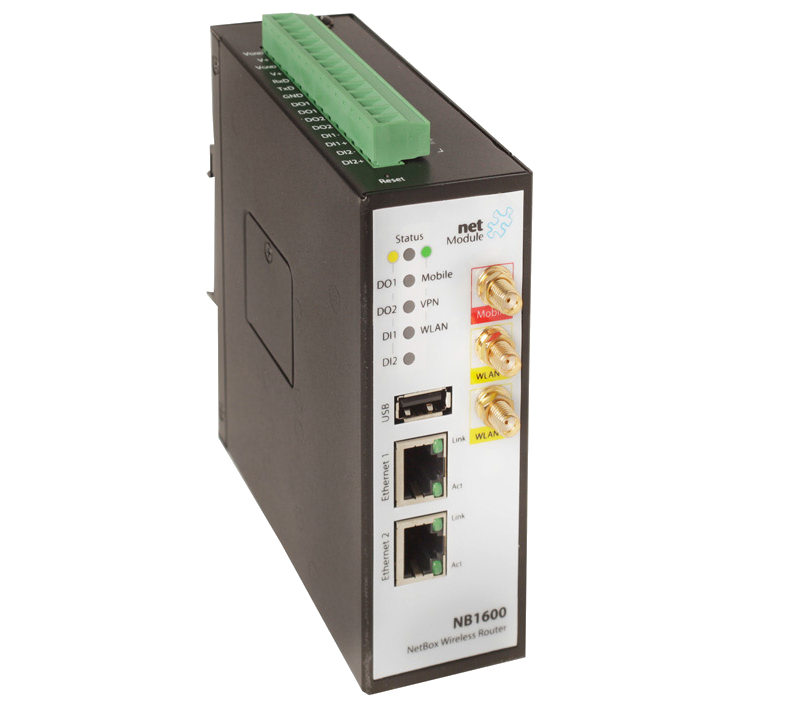
\includegraphics[width=6cm]{bilder/netmodule.png}
	\caption{Foto NetModule NB1600}
	\label{fig:netbox}
\end{figure}


\section{BeagleBone Black mit CAN-Cape}
Als Basis für unsere Software kommt ein BeagleBone Black als Recheneinheit zum Einsatz. Zum Anschliessen der drei CAN-Busse des Fahrzeuges verwenden wir ein von einem Italiener gefertigtes CAN-Cape, dass einfach auf das Beaglebone drauf gesteckt werden kann:

\begin{figure}[hbtp]
	\center
	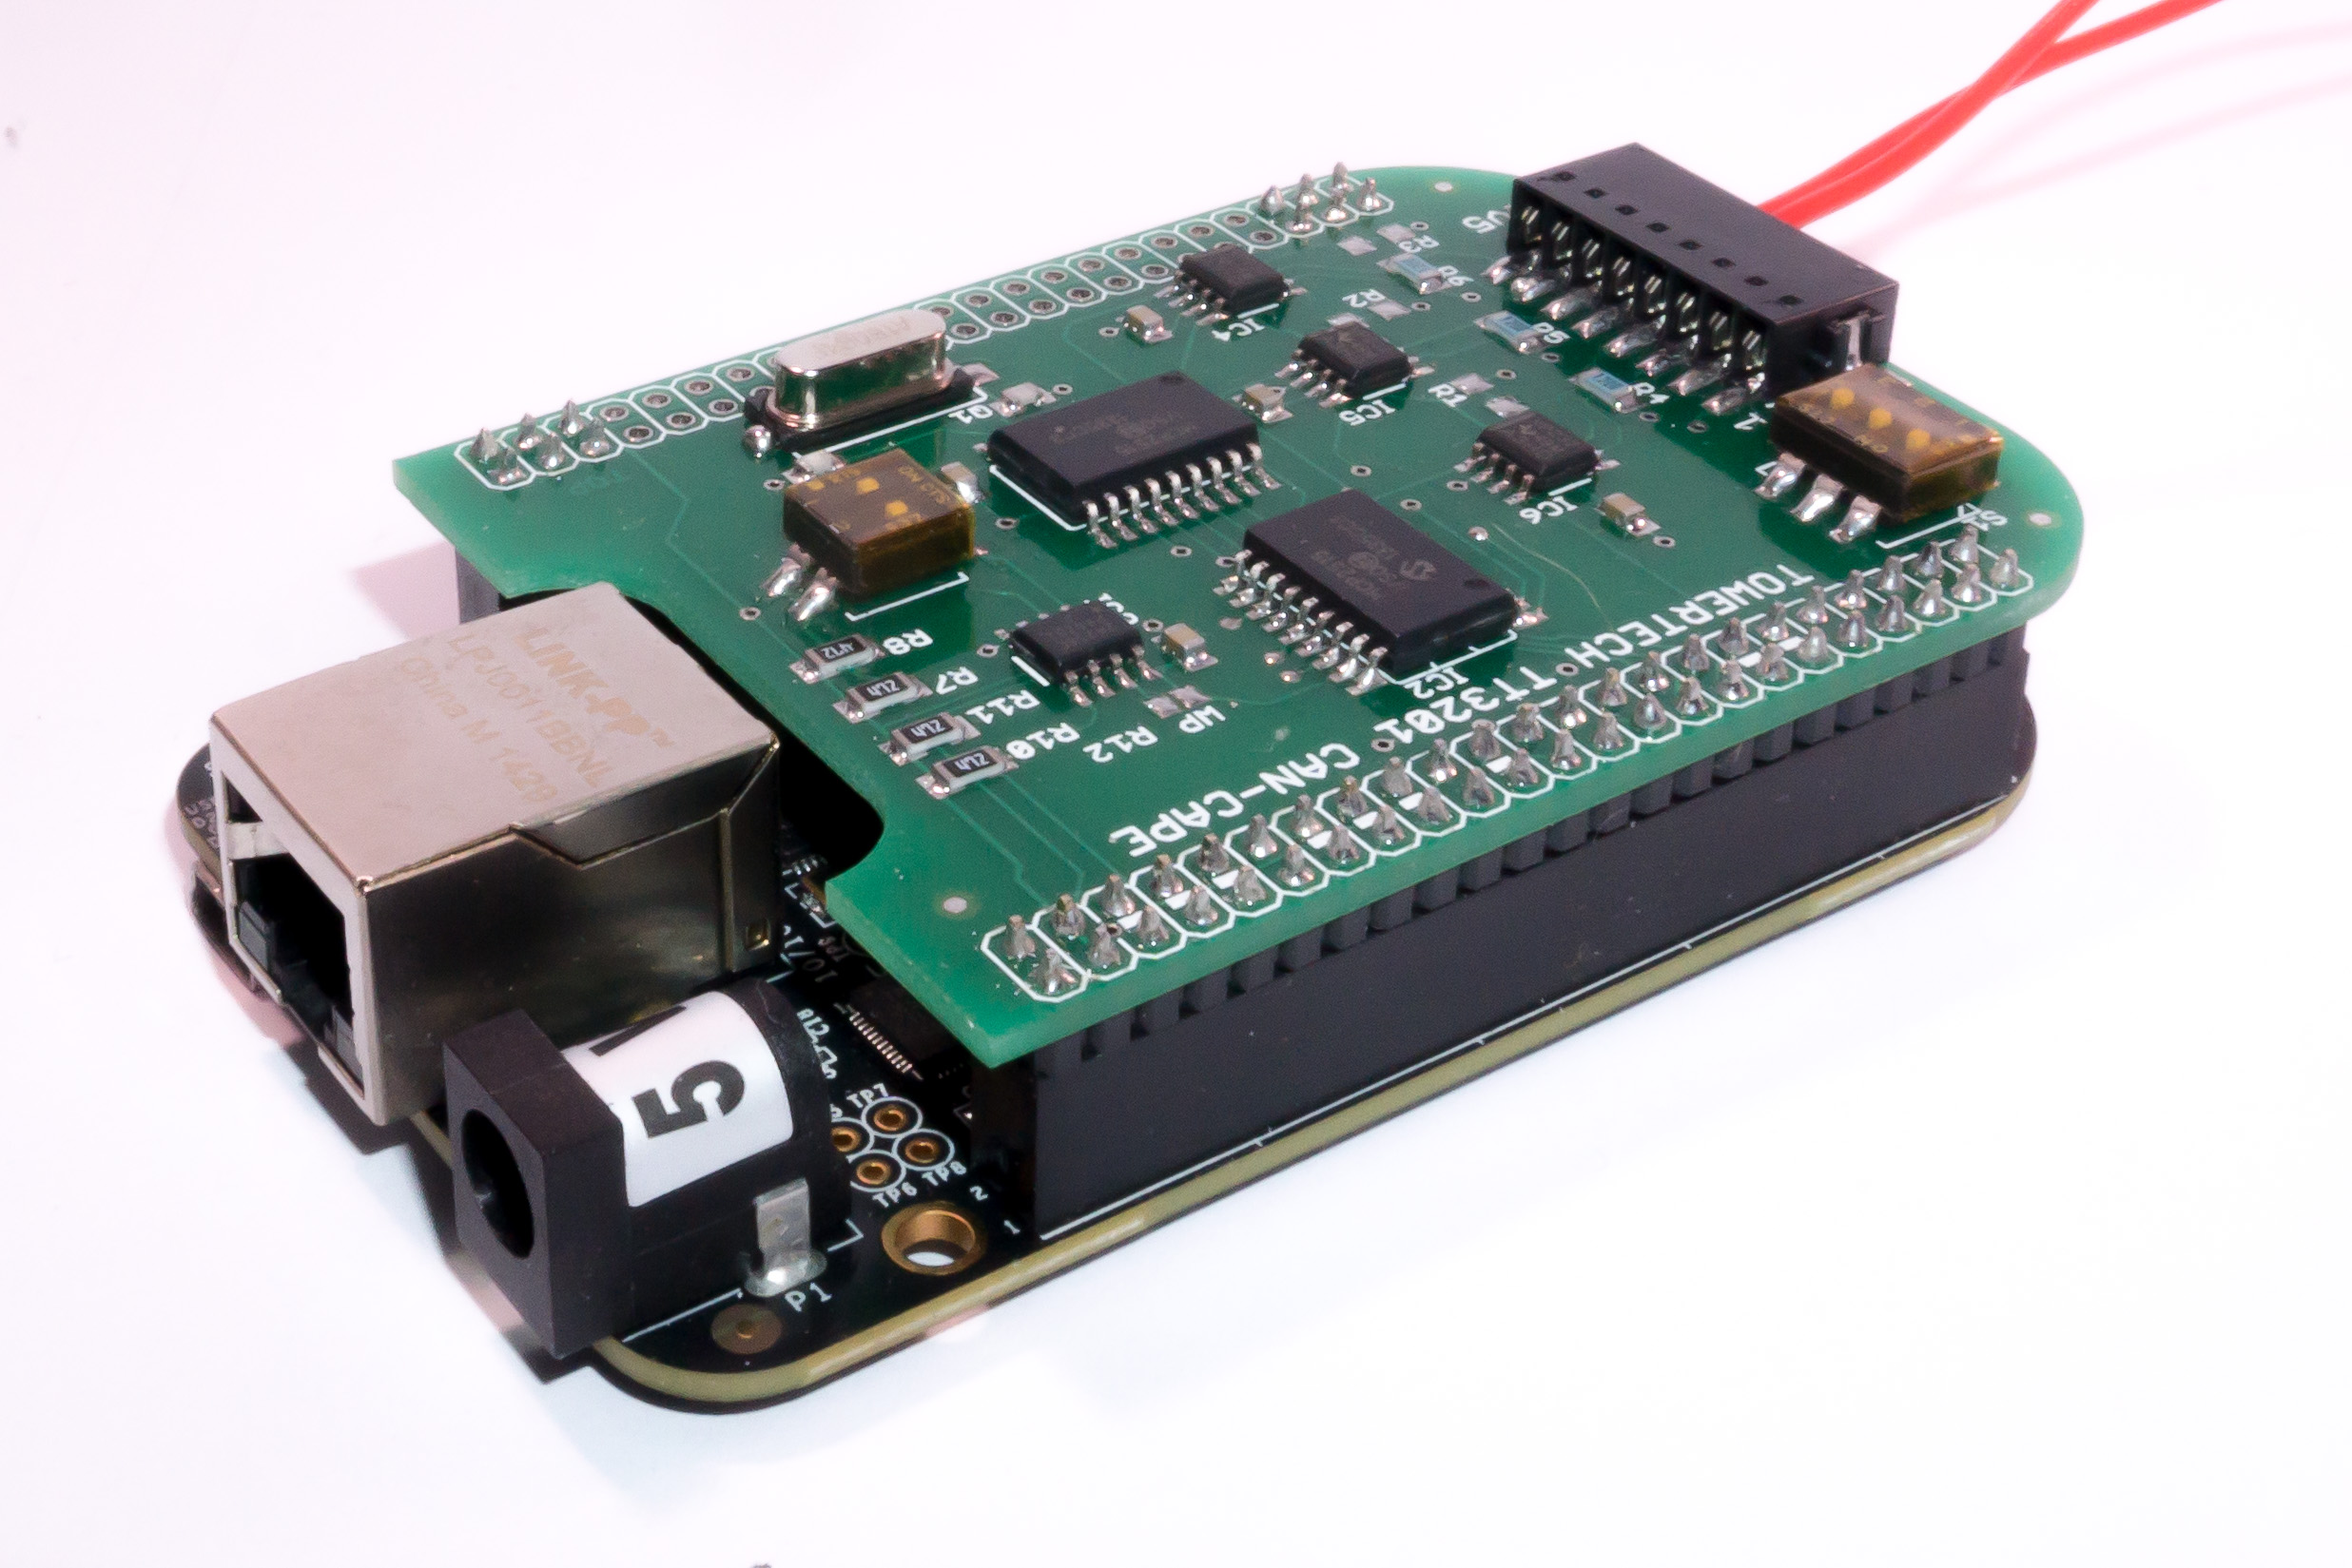
\includegraphics[width=\textwidth]{bilder/foto-4.jpg}
	\caption{Foto BLED112}
	\label{fig:bled112}
\end{figure}

\textbf{Installationsinstruktionen siehe Anhang.}

\subsection{BeagleBone Hardware Spezifikation}
\begin{itemize}
	\itemsep 1pt \parskip 0pt \parsep 0pt
	\item Prozessor:	AM335x 1GHz ARM® Cortex-A8
	\item RAM:			512MB DDR3 RAM
	\item HDD:			4GB 8-bit eMMC on-board flash storage
	\item GPU:  		3D graphics accelerator + NEON floating-point accelerator
	\item 2x PRU 32-bit microcontrollers
	\item USB client for power and communications (Ethernet over USB)
	\item USB host
	\item Ethernet
	\item HDMI
	\item 2x 46 pin headers (GPIO, I2C, SPI, UART, CAN, etc.)
	\item Betriebssysteme:
	\begin{itemize}
		\itemsep 1pt \parskip 0pt \parsep 0pt
		\item Debian
		\item Android
		\item Ubuntu
		\item Cloud9 IDE on Node.js w/ BoneScript library
		\item plus jedes weitere ARM kompatible Betriebssystem
	\end{itemize}		
\end{itemize}



\section{BLED112}

\begin{figure}[hbtp]
	\center
	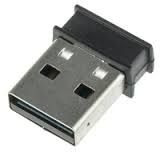
\includegraphics[width=4cm]{bilder/bled112.jpg}
	\caption{Foto BLED112}
	\label{fig:bled112}
\end{figure}

Die wichtigsten zu wissenden Details über den Bluegiga Dongle sind die folgenden:

\begin{itemize}
\itemsep 1pt \parskip 0pt \parsep 0pt
\item Kommunikation erfolgt über serielle Schnittstelle. Dem BLED112 werden darüber einfach die enstprechenden Anweisungen gesendet.

\item Material zu BLED112 (API Doku, Windows Treiber, Linux/Mac works out of the box) \url{https://www.bluegiga.com/en-US/products/bled112-bluetooth-smart-dongle/#documentation} → siehe im Speziellen API 1.3 Referenz


\item Java-LIB, wo die BLED 112 API bereits implementiert ist: \url{https://github.com/SINTEF-9012/bglib}


\item Ein paar Worte zum BLED112 selber:
	\begin{itemize}
	\itemsep 1pt \parskip 0pt \parsep 0pt
	\item  Das Teil ist programmierbarer Mikrocontroller mit komplett implementiertem Bluetooth-Stack, verpackt als USB-Dongle (Dongle = das D im BLED112)

	\item  Durch die Programmierung in Bluescript kann der Dongle unter anderem zu einem iBeacon gemacht werden.


	\item  Theoretisch bietet er aber viel mehr an. Er ist nebenbei ein direktes Konkurrenzprodukt zum nRF51 Chip von Nordic, der auf dem Sming zum Einsatz kommt.
	\end{itemize}


\item Beispiel-Befehlsabfolge, wie sie beim Sming zum Einsatz kommt. Detailbeschrieb der Parameter siehe Bluegiga API 1.3 Doku. Die Parameter-Werte entsprechen denen im Demo-Script und sollten lauffähig sein:

	\begin{itemize}
	\itemsep 1pt \parskip 0pt \parsep 0pt
	\item Suche nach BLE Advertisments
		\begin{itemize}
			\itemsep 1pt \parskip 0pt \parsep 0pt
			\item bg.api.gapSetScanParameters(0xC8, 0xC8, 0)
			\item bg.api.gapDiscover(1)
		\end{itemize}

	\item Wenn ein Device mit Name TXW51 gefunden, beende Suche kommt als Event mit Class = GenericAccessProfile siehe Demo-Script ab Zeile 238
		\begin{itemize}
			\itemsep 1pt \parskip 0pt \parsep 0pt
			\item Suche beenden: bg.api.gapEndProcedure()
		\end{itemize}
	

	\item Verbinde zum gefundenen Device anhand seiner MAC-Adresse
		\begin{itemize}
			\itemsep 1pt \parskip 0pt \parsep 0pt
			\item bg.api.gapConnectDirect( <MAC-Addr>, 1, 60, 76, 100, 9)
		\end{itemize}



	\item Hole einfach mal komplette Handle-Liste der Bluetooth Attribute (Optimieriungspotential da)
			\begin{itemize}
				\itemsep 1pt \parskip 0pt \parsep 0pt
				\item bg.api.attClientFindInformation( <connectionHandle>, 1, 0xffff)
			\end{itemize}


	\item Stimme die SMING UUIDs mit denen in der Handle-Liste überein. Merke zu jeder UUID deren Handle sowie UUID der CCID Attributes (siehe später)


	\item Lese mit den entsprechenden Handle das Attribut (ich habe einfach mal jeweils immmer gerade mal alle eingelesen)
			\begin{itemize}
				\itemsep 1pt \parskip 0pt \parsep 0pt
				\item bg.api.attClientReadByHandle(<connection>, <uuid handle> )
			\end{itemize}


	\item Zum Aktivieren der Accelometer-Messungen müssen folgende Attributte geschrieben werden:
			\begin{itemize}
				\itemsep 1pt \parskip 0pt \parsep 0pt
				\item bg.api.attClientAttributeWrite( <connection>, <uuid handle>, <newValue>)
				\item \url{LSM330_CHAR_GYRO_EN} = 1 
				\item \url{LSM330_CHAR_ACC_EN} = 1 
				\item \url{CCID UUID 0x02, 0x29 = 0x01, 0x00} ( Dies aktiviert das Bluetooth Feature CCID, wodruch das Sming bei Sming seitiger Attributwertänderung automatisch den neuen Wert sendet. Die Messwerte werden so per Push übertragen. Seitens Sming wird somit einfach der Messwert auf das Attribut \url{MEASURE_CHAR_DATASTREAM} geschrieben. Dies löst aus, dass der Bluetooth Stack des Smings automatisch den neue Messwert als Event zum Bluegiga Dongle übertragt und wir das so mitkriegen)
				\item \url{MEASURE_CHAR_START} = 1
			\end{itemize}


	\item Das Lesen der Temperatur muss mit einem Polling auf Attribut \url{LSM330_CHAR_TEMP_SAMPLE} gemacht werden.

	\item Beende Verbindung zum Sming
			\begin{itemize}
				\itemsep 1pt \parskip 0pt \parsep 0pt
				\item bg.api.connectionDisconnect( <connection> )
			\end{itemize}
	\end{itemize}
\end{itemize}


\chapter{SMING}\label{sec:sming}
Um weitere Sensoren einfach ohne Verdrahtung ins Messsystem aufzunehmen, setzen wir auf das Sming. Das Sming wurde durch Daniel Meer in seiner Master Thesis entwickelt. Er beschreibt in der Thesis das Sming wie folgt: \textit{Der TXW51 ist ein kleiner und energiesparender Sensorknoten, der als Basis für zukünftige Projekte verwendet werden kann. Er kommuniziert über Bluetooth Smart und enthält einen Sensor zur Messung der Beschleunigung. Die Firmware kann einfach für neue Anforderungen modifiziert werden.}\cite{meer:masterthesis}

\begin{figure}[hbtp]
	\center
	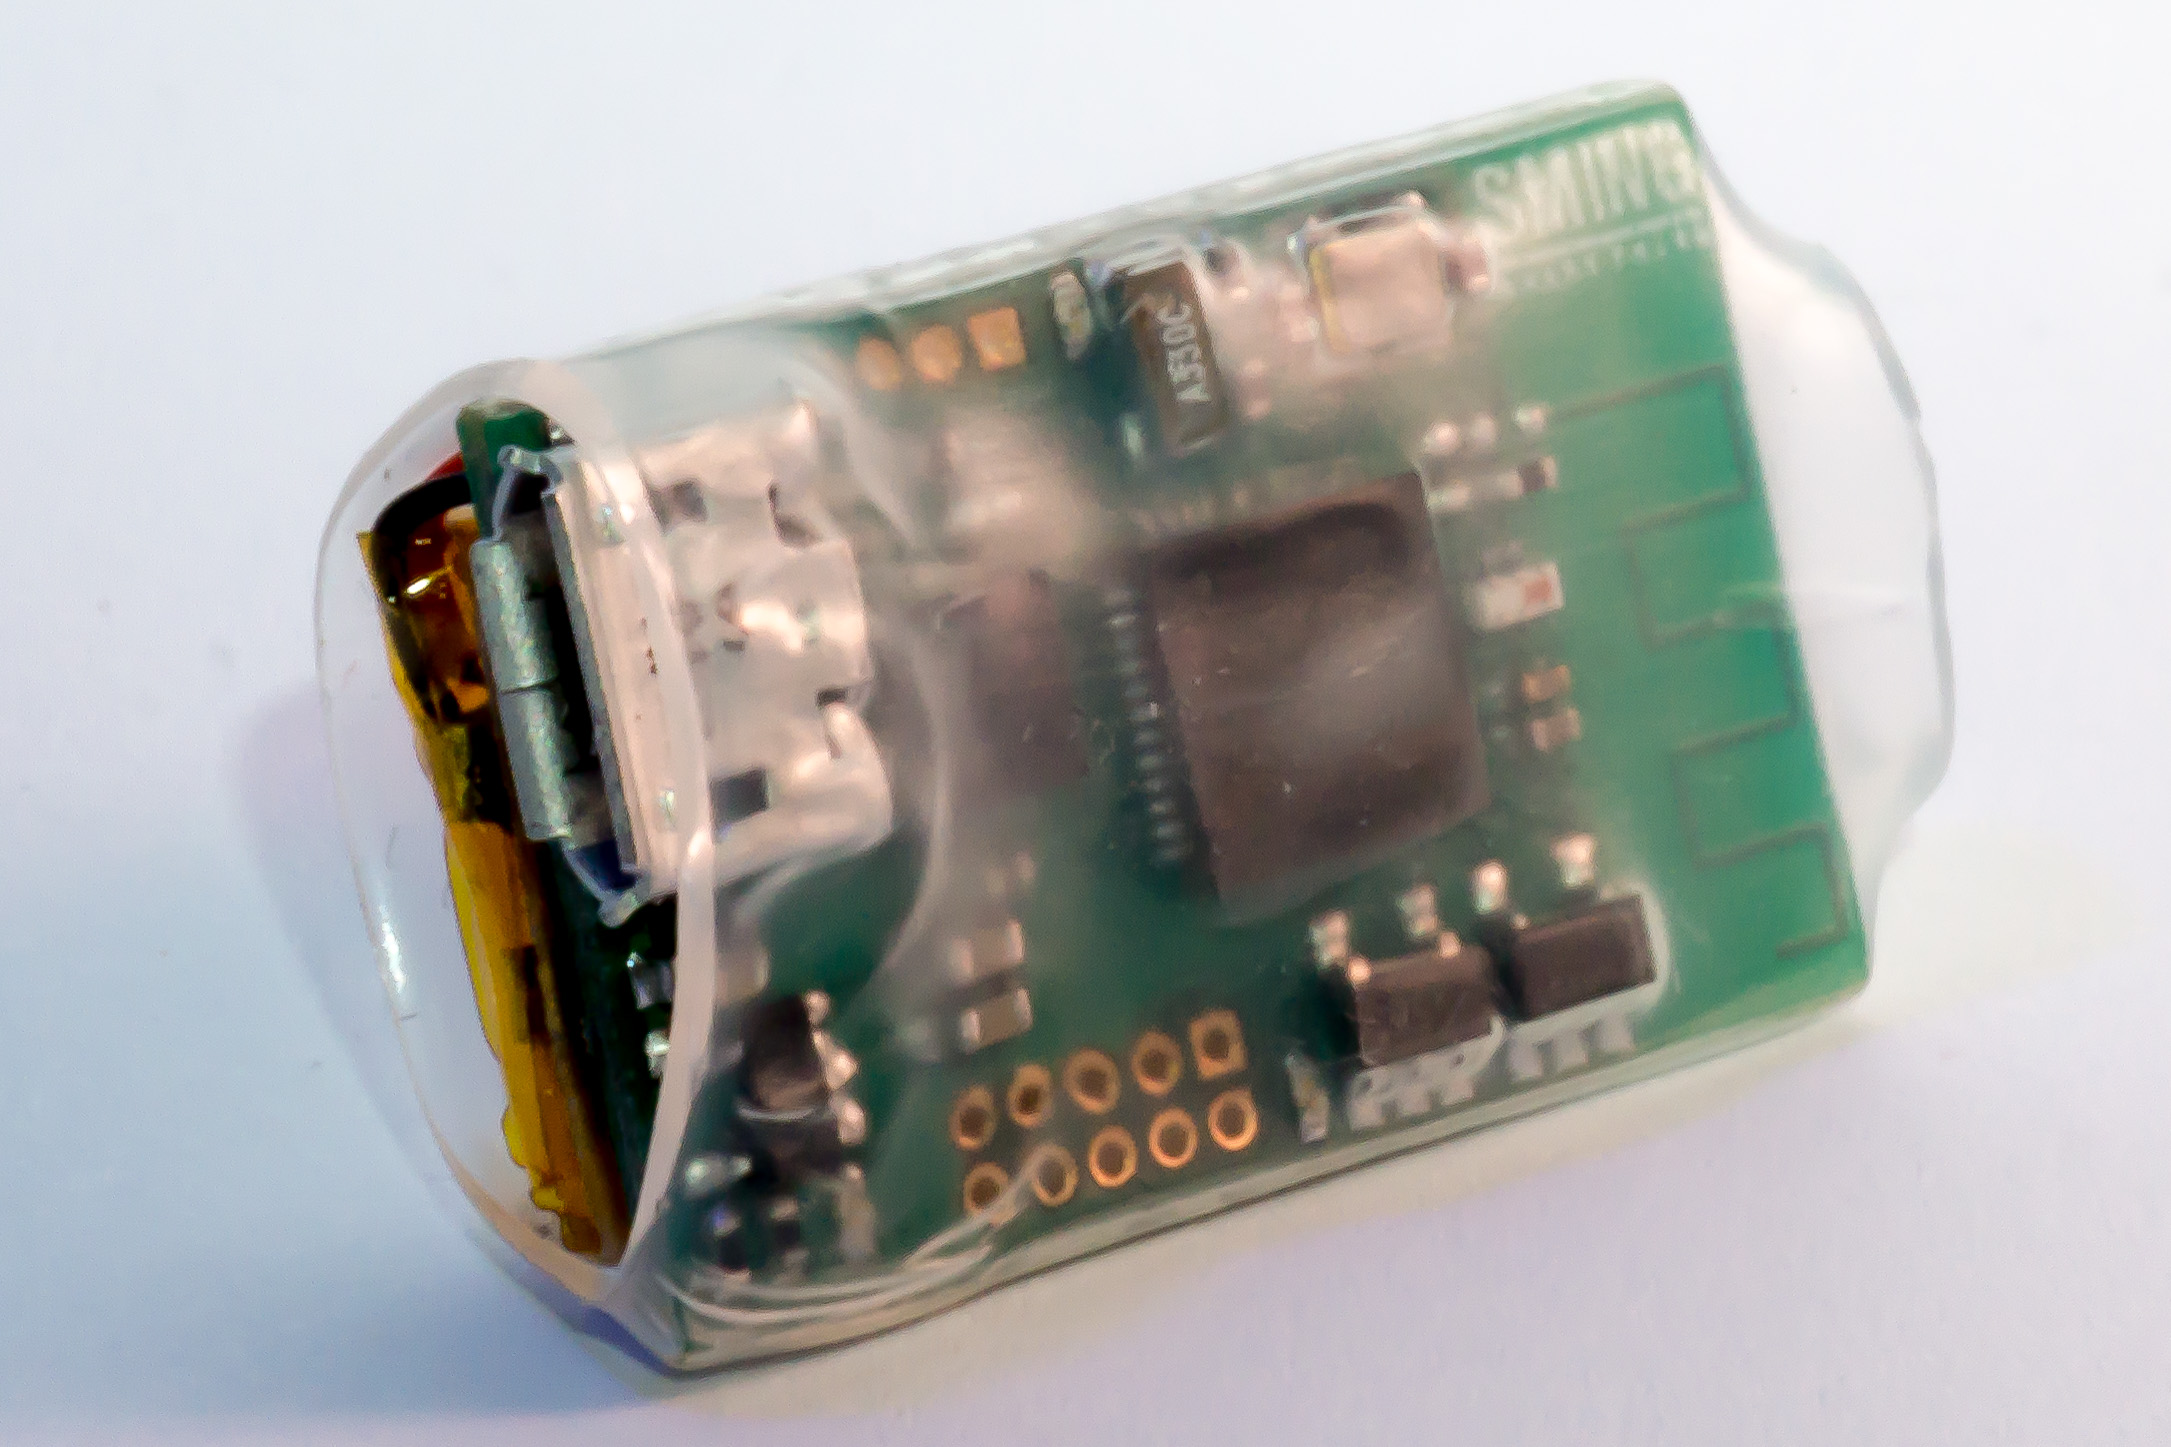
\includegraphics[width=10cm]{bilder/foto-6.jpg}
	\caption{Foto Sming mit Akku bestückt}
	\label{fig:sming}
\end{figure}

Für unser Projekt ist vorallem die Erweiterbarkeit des Sming sehr interessant. Dies weil beliebige Senosoren über I2C angesprochen werden können.

Hier nochmals die wichtigsten Eigenschaften:

\begin{itemize}
	\itemsep 1pt \parskip 0pt \parsep 0pt
	\item Kommunikation über Bluetooth 4.0
	\item Werte werden über BLE GATT gelesen und geschrieben 
	\item Speziell wissenswert: Messungen werden per PUSH über Bluetooth CCID Feature gesendet, Details siehe Beschreibung BLED112
	\item Bluetooth Device Name ist bei allen Smings von der BFH Burgdorf:  TXW51
	\item Grundsätzlich sind die Attribute des SMINGS in drei Gruppen unterteilbar:
	\begin{itemize}
		\itemsep 1pt \parskip 0pt \parsep 0pt
		\item Beginnend mit \url{DEVICE_INFO}: diverse einfache Textfelder, die auch selber nach gutdünken beschrieben werden können.
		\item Beginnend mit LSM330: Die entsprechenden Einstellung und Werte des LSM330-Sensors (Kombinierter Gyro-,Accelometer- und Temperatur-Sensor)
		\item Beginnend mit MEASURE: Die entsprechenden Funktionen, um die asynchrone Messung via Bluetooth Push zu konfigurieren (Dauer), zu starten, zu stoppen und auch von Hand den letzten Messwert abzufragen.
		
	\end{itemize}
	\item Tipp: Über das Demo-Tool von Bluegiga kann händisch mit dem SMING verbunden und Attribute gelesen/geschrieben werden.
	
	\item Messwert-Attribut: Zum Optimieren der Performance sind auf dem Messwert-Attribut oft bis zu drei Messwerte binär aneinandergereit vorhanden. Das Decodieren des Wertes wird im Demo-Script von Zeile 319 bis 345 gemacht.
	
	\item Java-Beispielcode für Kommunikation ist ebenfalls vorhanden,siehe gezippter Source der Demo-Android App von Daniel Meer auf Google Drive. Dort wird aber mit den Android Bluetooth Stack gearbeitet und nicht mit dem Bluegiga, weswegen sich das leider nicht ganz eins zu eins kopieren lässt. 
	
	\item Hinweis: das CCID wird von Android im Gegensatz zu Bluegiga als Funktion abstrahiert.
\end{itemize}

\subsection{Liste der wichtigsten Attribut UUIDs}
\begin{lstlisting}
DEVICE_INFO_SERVICE           : "8EDF0100-67E5-DB83-F85B-A1E2AB1C9E7A",
DEVICE_INFO_CHAR_MANUFACTURER : "8EDF0101-67E5-DB83-F85B-A1E2AB1C9E7A",
DEVICE_INFO_CHAR_MODEL        : "8EDF0102-67E5-DB83-F85B-A1E2AB1C9E7A",
DEVICE_INFO_CHAR_SERIAL       : "8EDF0103-67E5-DB83-F85B-A1E2AB1C9E7A",
DEVICE_INFO_CHAR_HW_REV       : "8EDF0104-67E5-DB83-F85B-A1E2AB1C9E7A",
DEVICE_INFO_CHAR_FW_REV       : "8EDF0105-67E5-DB83-F85B-A1E2AB1C9E7A",
DEVICE_INFO_CHAR_DEVICE_NAME  : "8EDF0106-67E5-DB83-F85B-A1E2AB1C9E7A",
DEVICE_INFO_CHAR_SAVE_VALUES  : "8EDF0107-67E5-DB83-F85B-A1E2AB1C9E7A",

LSM330_SERVICE           : "8EDF0200-67E5-DB83-F85B-A1E2AB1C9E7A",
LSM330_CHAR_ACC_EN       : "8EDF0201-67E5-DB83-F85B-A1E2AB1C9E7A",
LSM330_CHAR_GYRO_EN      : "8EDF0202-67E5-DB83-F85B-A1E2AB1C9E7A",
LSM330_CHAR_TEMP_SAMPLE  : "8EDF0203-67E5-DB83-F85B-A1E2AB1C9E7A",
LSM330_CHAR_ACC_FSCALE   : "8EDF0204-67E5-DB83-F85B-A1E2AB1C9E7A",
LSM330_CHAR_GYRO_FSCALE  : "8EDF0205-67E5-DB83-F85B-A1E2AB1C9E7A",
LSM330_CHAR_ACC_ODR      : "8EDF0206-67E5-DB83-F85B-A1E2AB1C9E7A",
LSM330_CHAR_GYRO_ODR     : "8EDF0207-67E5-DB83-F85B-A1E2AB1C9E7A",
LSM330_CHAR_TRIGGER_VAL  : "8EDF0208-67E5-DB83-F85B-A1E2AB1C9E7A",
LSM330_CHAR_TRIGGER_AXIS : "8EDF0209-67E5-DB83-F85B-A1E2AB1C9E7A",

MEASURE_SERVICE         : "8EDF0300-67E5-DB83-F85B-A1E2AB1C9E7A",
MEASURE_CHAR_START      : "8EDF0301-67E5-DB83-F85B-A1E2AB1C9E7A",
MEASURE_CHAR_STOP       : "8EDF0302-67E5-DB83-F85B-A1E2AB1C9E7A",
MEASURE_CHAR_DURATION   : "8EDF0303-67E5-DB83-F85B-A1E2AB1C9E7A",
MEASURE_CHAR_DATASTREAM : "8EDF0304-67E5-DB83-F85B-A1E2AB1C9E7A"
\end{lstlisting}
